\section{Régression logistique}
\subsection{Affichage des données}

\begin{figure}[!h]
    \begin{minipage}{.40\linewidth}
            Une première fonction \textit{plotData()}, qui permet d'afficher un graphique 2D avec les axes représentant les deux notes des examens, et les exemples positifs et négatifs affichés avec différents marqueurs. \\
            L'objectif de cette partie sera de construire un modèle de régression logistique pour prédire si un étudiant est admis dans une université en comprenant sa méthodologie.
    \end{minipage}\hfill
    \begin{minipage}{.56\linewidth}
        \begin{center}
            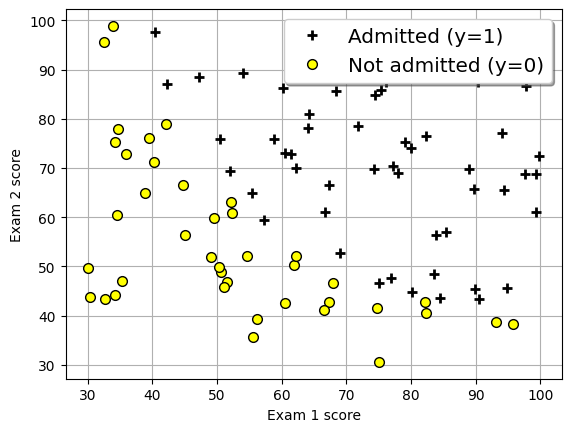
\includegraphics[width=1\textwidth]{./img/3.1.png}
            \caption{\label{fig:fig1}Diagramme de dispersion des données d'entraînement}  
        \end{center}
    \end{minipage}
\end{figure}

\begin{figure}[!h]
\begin{minted}[frame=lines, framesep=2mm, baselinestretch=1.2, fontsize=\footnotesize, linenos, breaklines=true]{python}
def plotData(X,y):
    pos = X[(y==1).flatten(),:]
    neg = X[(y==0).flatten(),:]
    plt.plot(pos[:,0], pos[:,1], '+', markersize=7, markeredgecolor='black', markeredgewidth=2) 
    plt.plot(neg[:,0], neg[:,1], 'o', markersize=7, markeredgecolor='black', markerfacecolor='yellow') 
    plt.legend(['Admitted (y=1)', 'Not admitted (y=0)'], loc='upper right', shadow=True, fontsize='x-large', numpoints=1) 
    plt.grid()
    plt.xlabel('Exam 1 score')
    plt.ylabel('Exam 2 score')
\end{minted}   
\captionof{listing}{Fonction plotData}
\end{figure}

    \subsection{Implémentation}

    Le modèle de régression linéaire est représenté par l'équation \ref{eq:regression_linear}. Cette équation nous permet d'obtenir une prédiction en fonction d'une entrée~$x$ et de $\theta$.
    
\begin{figure}[!h]
    \begin{minipage}{.48\linewidth}
\begin{minted}[frame=lines, framesep=2mm, baselinestretch=1.2, fontsize=\footnotesize, linenos, breaklines=true]{python}
def sigmoid(z):
        g = 1 / (1 + np.exp(-z))

    return  g
\end{minted}   
    \end{minipage}\hfill
    \begin{minipage}{.48\linewidth}
        \begin{align}\label{eq:regression_linear}
            h_\theta(x) = g (x^T \theta ) \\
            g(z)=\frac{1}{1-e^{-z}} 
        \end{align}
\end{minipage}
\end{figure}
    
    \noindent
    Pour que cette prédiction soit optimale, il est important de déterminer correctement les paramètres de notre modèle~: $\theta$. Pour cela, nous devons réaliser deux étapes~: Le calcul du coût $J(\theta)$ et une descente de gradient.

    \subsubsection{Calcul du coût $J(\theta)$}
    De la même manière que dans le TP1, le calcul du coût $J(\theta)$ permet de mesurer la qualité de la prédiction, si le coût est faible alors notre prédiction est proche des valeurs réelles et inversement si le coût est important. La formule utilisée pour calculer ce coût n'est pas la même pour une régression linéaire que pour une régression logistique. 
    
    \begin{equation}\label{eq:cout}
       J(\theta) = \frac{1}{m} \sum_{i=0}^{m-1}[-y^{(i)} log(h_\theta(x^{(i)})) - (1-y^{(i)}) log(1-h_\theta(x^{(i)}))]
    \end{equation}
 
    On remarque ici avec l'équation \ref{eq:cout} qui utilise l'équation \ref{eq:regression_linear}, que la seule valeur qui puisse influencer notre coût est $\theta$. Effectivement, les valeurs restantes : $x$, $y$ et $m$; sont les valeurs
    de notre problème qui sont déterminées et non modifiables.
    
    
    \vspace{.5cm}
    \noindent
    \textbf{Mise en application}
    \vspace{.2cm}

\begin{figure}[!h]
\begin{minted}[frame=lines, framesep=2mm, baselinestretch=1.2, fontsize=\footnotesize, linenos, breaklines=true]{python}
def costFunction(theta, X, y):
    # Initialize some useful values
    m,n = X.shape   
    theta = theta.reshape((n,1)) 
                
    predictions = sigmoid(X @ theta)
    J = (1/m) * np.sum(-y * np.log(predictions) - (1 - y) * np.log(1 - predictions))
    
    return  J

    """ return
    Cost at initial theta (zeros): 0.693147
    Expected cost (approx): 0.693
    """
\end{minted}   
\captionof{listing}{Fonction computeCost}
\end{figure}

\clearpage

\subsubsection{Descente de gradient}

La descente de gradient permet de minimiser le coût et donc d'obtenir les bonnes valeurs de theta pour réaliser une prédiction optimale.

\begin{equation}\label{eq:descente-gradient}
    \frac{\partial J(\theta)}{\partial \theta_j} = \frac{1}{m} \sum_{i=1}^{m} (h_\theta(x^{(i)}) - y^{(i)}) x_j^{(i)}
\end{equation}

\noindent
 Le calcul du gradient de la régression logistique comme pour le coût n'est pas identique à celle de la régression linéaire, en effet cela est dû aux définitions différentes de \( h_\theta (x) \).

\vspace{.5cm}
    \noindent
    \textbf{Mise en application}
    \vspace{.2cm}

\begin{figure}[!h]
\begin{minted}[frame=lines, framesep=2mm, baselinestretch=1.2, fontsize=\footnotesize, linenos, breaklines=true]{python}
def gradientFunction(theta, X, y):
    m = X.shape[0]  
    n = X.shape[1]   
    theta = theta.reshape((n,1)) 
    grad = 0
    for i in range(m):
        grad += (1/m) * (sigmoid(X[i] @ theta) - y[i]) * X[i]
    return grad

    """ return 
    theta: ['-25.1613', '0.2062', '0.2015']
    Expected theta (approx): -25.161 0.206 0.201
    For a student with scores 45 and 85, we predict an admission probability of 0.776291
    Expected Proba (approx): 0.776
    Train Accuracy: 89.000000
    Expected accuracy (approx): 89.0%"""
\end{minted}   
\captionof{listing}{Fonction gradientFunction}
\end{figure}

\subsubsection{La fonction d'optimisation fmin\_tnc}

La fonction d'optimisation \textit{fmin\_tnc} nous permet d'obtenir automatiquement les $\theta$ minimisés sans donner de valeurs test. 

\begin{figure}[!h]
\begin{minted}[frame=lines, framesep=2mm, baselinestretch=1.2, fontsize=\footnotesize, linenos, breaklines=true]{python}
theta = opt.fmin_tnc(costFunction, initial_theta, gradientFunction, args=(X, y))[0]
cost = costFunction(theta, X, y)  
print('Cost at theta found by scipy: %f' % cost)
print('Expected cost (approx): 0.203')
print('theta:', ["%0.4f" % i for i in theta])
print('Expected theta (approx): -25.161 0.206 0.201')

""" result
Cost at theta found by scipy: 0.203498
Expected cost (approx): 0.203
theta: ['-25.1613', '0.2062', '0.2015']
Expected theta (approx): -25.161 0.206 0.201"""
\end{minted}   
\captionof{listing}{fmin\_tnc}
\end{figure}

\subsection{Évaluation de la régression logistique}

Pour rappel la fonction \textit{sigmoid} représente la prédiction, donc l'appel de sigmoid avec notre $\theta$ minimisé doit nous permettre d'obtenir une prédiction fiable.  \\
Si notre prédiction est supérieur à 1, cela signifie que l'étudiant est admis. \\
Si on suit cette logique la fonction suivante nous permet d'obtenir la prédiction des élèves admis et non-admis, on peut donc tracer la limite de décision.


\begin{figure}[!h]
    \begin{minipage}{.40\linewidth}
\begin{minted}[frame=lines, framesep=2mm, baselinestretch=1.2, fontsize=\footnotesize, linenos, breaklines=true]{python}
def predict(theta, X):
    return (sigmoid(X @ theta) >= 0.5).astype(int)
\end{minted}   
\captionof{listing}{Fonction gradientFunction}
    \end{minipage}\hfill
    \begin{minipage}{.56\linewidth}
        \begin{center}
            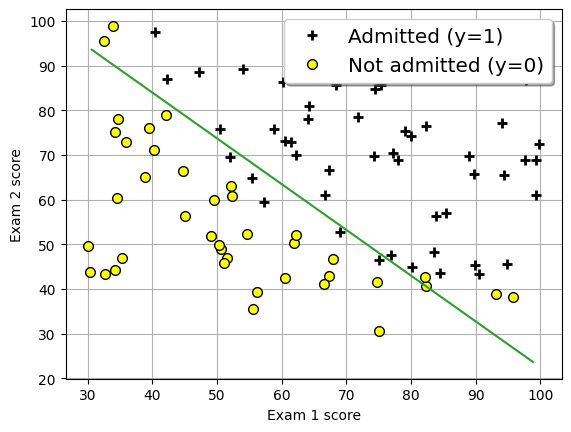
\includegraphics[width=1\textwidth]{./img/3.2.png}
            \caption{\label{fig:3.2}Limite de décision}  
        \end{center}
    \end{minipage}
\end{figure}